\documentclass[10pt,a4paper,twocolumn]{article}
\usepackage[utf8]{inputenc}
\raggedbottom
\usepackage[english]{babel}
\usepackage{amsmath}
\usepackage{amsfonts}
\usepackage{amssymb}
\usepackage{graphicx}
\usepackage{multicol}
\setlength{\columnsep}{1cm}
\usepackage[left=2cm,right=2cm,top=2cm,bottom=2cm]{geometry}
\author{N Praful Raj}
\title{\textbf{Assignment-1}}
\numberwithin{equation}{section}
\graphicspath{ {./images/} }
\begin{document}
\maketitle
%\begin {multicols}{1}



	
\section{Problem}
Find the coordinates of the point where the line through$\begin{pmatrix}3 \\-4 \\-5\end{pmatrix}$ and $\begin{pmatrix}2 \\-3 \\1\end{pmatrix}$ crosses the plane $\begin{pmatrix}2 & 1 & 1\end{pmatrix}$x=7 

\section{Explanation}\label{exp}
We know that vector equation of line passing through two points , say A and B is
\begin{gather}\label{lineeqn}\textbf{x} = \vec{A}+\lambda\begin{pmatrix}\vec{B}-\vec{A}\end{pmatrix}
\end{gather}
We also know that equation of a plane is \begin{gather}\label{plane}\textbf{n}^T\textbf{x}=c\end{gather}
Substituting \ref{lineeqn} in \ref{plane} as line passes through the plane we can get the point of contact.

\section{Solution}
\textbf{Step 1}\\
Let us first findout the equation of line passing through two given points using \ref{lineeqn} \\
\\\begin{gather}\textbf{x}=\begin{pmatrix}3 \\-4 \\-5\end{pmatrix}+\lambda 
\begin{pmatrix}2-3 \\-3+4 \\1+5\end{pmatrix}\end{gather}
\\
\begin{gather}\label{lineq1}
% \vec{r}=(-\lambda +3)\hat{i}+(\lambda - 4)\hat{j}+(6 \lambda - 5)\hat{k}
\textbf{x}=\begin{pmatrix}3 \\-4 \\-5\end{pmatrix}+\lambda 
\begin{pmatrix}-1 \\1 \\6\end{pmatrix}
\end{gather}
\textbf{Step 2}\\
Now let us construct the equation of plane from the given data.\\
Using the values we can construct 
\begin{gather}\label{n}
%\hat{n}= \dfrac{2\hat{i}+\hat{j}+\hat{k}}{\sqrt{6}}
\textbf{n}=\begin{pmatrix} 2\\ 1\\1\end{pmatrix}
\end{gather}\\
%\begin{gather}\label{d}d=\dfrac{|7|}{\sqrt{6}}\end{gather}

\textbf{Step 3}\\
Now using \ref{lineq1} , \ref{n}   in \ref{plane}\\

\begin{gather}\label{r1}
%\bigg( (-\lambda +3)\hat{i}+(\lambda - 4)\hat{j}+(6 \lambda - 5)\hat{k} \bigg) \cdot \bigg( \dfrac{2\hat{i}+\hat{j}+\hat{k}}{\sqrt{6}} \bigg) = \dfrac{|7|}{\sqrt{6}}
\textbf{n}^T\textbf{x}=c
%\begin{pmatrix} 2 && 1 && 1\end{pmatrix} \Bigg( \begin{pmatrix}3 \\-4 \\-5\end{pmatrix}+\lambda\begin{pmatrix}-1 \\1 \\6\end{pmatrix} \Bigg)=7
\end{gather}
solving \ref{r1} we get \\
\begin{gather}  6 -4 -5-2\lambda+ \lambda+ 6 \lambda=7 \end{gather}
\\ \begin{gather} 5 \lambda=10 \end{gather}
\begin{gather}\label{la} 
\lambda=2 
\end{gather}
Now substituting the value of $\lambda$ in \ref{lineeqn} we get 
\begin{gather}\textbf{x}=\begin{pmatrix}-2+3\\2-4\\12-5 \end{pmatrix}\end{gather}
\\Therefore the point of contact of line on plane is
\\\begin{gather}\textbf{x}=\begin{pmatrix}1\\-2\\7 \end{pmatrix}\end{gather}
\pagebreak

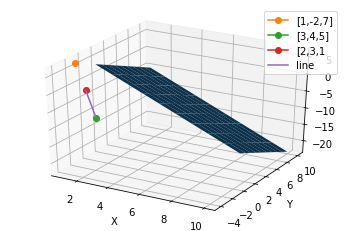
\includegraphics{Figure_3}
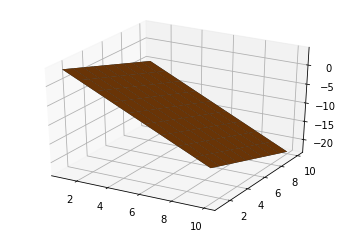
\includegraphics{Figure_4}






%\end{multicols}

\end{document}